\section{Gaussian Splatting}
\label{gaussian_splatting}

En el marco de este trabajo empleamos una técnica particular llamada \emph{Gaussian Splatting}. Esta técnica fue presentada en 2023 por Kerbl et al.~\cite{kerbl2023gaussian} y propone una representación explícita del entorno basada en un conjunto finito de densidades gaussianas tridimensionales. A diferencia de métodos implícitos como los campos de radiancia neuronales (NeRF), Gaussian Splatting describe la escena mediante primitivas geométricas, permitiendo un renderizado más eficiente.

Formalmente, la escena se modela como un conjunto de $N$ gaussianas tridimensionales
$$
\mathcal{G} = \{ g_i \}_{i=1}^N,
$$
donde cada gaussiana $g_i$ está caracterizada por su media $\boldsymbol{\mu}_i \in \mathbb{R}^3$, una matriz de covarianza $\boldsymbol{\Sigma}_i \in \mathbb{R}^{3 \times 3}$ que define su forma anisotrópica, un color $\mathbf{c}_i \in \mathbb{R}^3$ y un coeficiente de opacidad $\alpha_i \in [0,1]$. Esta parametrización permite capturar tanto la geometría como la apariencia de la escena de manera unificada.

Dado que la matriz de covarianza representa la dispersión de una variable aleatoria, debe ser simétrica y semidefinida positiva. Para garantizar esta propiedad y facilitar su interpretación geométrica, se parametriza la covarianza mediante una descomposición en rotación y escala.

En particular, se escribe:
\begin{equation}
\boldsymbol{\Sigma}
=
\mathbf{R}\,\mathbf{S}\,\mathbf{S}^\top\,\mathbf{R}^\top,
\end{equation}
donde \(\mathbf{R} \in SO(3)\) es una matriz de rotación ortonormal que define la orientación principal de la distribución, y \(\mathbf{S}\) es una matriz diagonal que contiene las desviaciones estándar a lo largo de los ejes principales.

Dado que es de la forma $\mathbf{A}\mathbf{A}^T$ para $\mathbf{A}=\mathbf{R}\mathbf{S}$, esta parametrización garantiza que \(\boldsymbol{\Sigma}\) sea siempre una matriz de covarianza válida. Geométricamente, esta descomposición define un elipsoide de incertidumbre cuya orientación está dada por \(\mathbf{R}\) y cuyos semiejes están determinados por los valores de \(\mathbf{S}\).




Sea $\pi$ la operación proyección, $\mu_i$ la posición de la gaussiana $i$ en coordenadas globales y $T_{wc}$ la transformación afín de coordenadas globales $w$ a coordenadas locales de la cámara $c$.
La proyección linealizada de una gaussiana multivariada a cualquier espacio de dimensión menor es una gaussiana. Manteniendo fijos el color y la opacidad, veamos cuáles son la media y covarianza de la gaussiana 2D, $\mu_i'$ y $\Sigma_i'$, respectivamente.

Al proyectar la Gaussiana 3D a una 2D, decimos que se propaga la covarianza. Debido a que la proyección es no lineal, trabajamos con una versión linealizada alrededor de la media $\mu_c$ truncando el polinomio de Taylor, siguiendo los pasos de \cite{zwicker2002ewa}

\begin{equation}
\pi(\mathbf{x}_c)
\approx
\pi(\boldsymbol{\mu}_c)
+
\mathbf{J}
\left(\mathbf{x}_c - \boldsymbol{\mu}_c\right),
\end{equation}

Utilizando propiedades de la probabilidad en matrices, dada una transformación lineal del tipo:
\begin{equation}
\mathbf{y} = \mathbf{A}\mathbf{x} + \mathbf{B}
\end{equation}

vale que la covarianza

\begin{equation}
\boldsymbol{\Sigma}_y = \mathbf{A}\boldsymbol{\Sigma}_x\mathbf{A}^\top.
\end{equation}

Luego,

\begin{equation}
\boldsymbol{\Sigma}'
=
\mathbf{J}\,\boldsymbol{\Sigma}_c\,\mathbf{J}^\top.
\end{equation}

Por la misma propiedad, y recordando que la covarianza en el sistema de referencia de la cámara es

\begin{equation}
\boldsymbol{\Sigma}_c
=
\mathbf{R}\,\boldsymbol{\Sigma}\,\mathbf{R}^\top
\end{equation}

tenemos que

\begin{equation}
\boxed{
\boldsymbol{\Sigma}'
=
\mathbf{J}\,\mathbf{R}\,\boldsymbol{\Sigma}\,\mathbf{R}^\top\,\mathbf{J}^\top
}
\end{equation}

Notemos que $\boldsymbol{\Sigma}' \in \mathbb{R}^{3\times 3}$, sin embargo, la covarianza de la gaussiana 2D se puede extraer salteándonos la última fila y columna.

Para la media $\mu_i'$, basta con proyectar la media original en el sistema de referencia de la cámara. Esto es,
$\mu_i' = \pi(\mathbf{T}_{cw} \cdot  \mu_i)$.

A partir de la media y la matriz de covarianza, podemos determinar nuestra gaussiana respecto de la densidad $\alpha$, siguiendo una variación de la fórmula probabilística clásica:

\begin{equation}
\alpha_i(x) = o_i \cdot e^{-\frac{1}{2}(x-\mu_i')^T \Sigma_i'^{-1}(x-\mu_i')}
\end{equation}

Notemos que el término de normalización de la gaussiana, que multiplica la exponencial, no está definido. Esto se debe a que no empleamos la gaussiana desde el punto de vista de la probabilidad sino como primitiva. Al tener control sobre el término multiplicativo, ganamos un grado de libertad en la representación. En su lugar, tenemos un término de opacidad, que se optimizará junto al resto de parámetros.




\subsection{Renderizado}

El proceso de renderizado consiste en proyectar cada gaussiana del espacio tridimensional al plano de la imagen utilizando el modelo de cámara pinhole y la pose de la cámara. Bajo esta proyección, cada gaussiana 3D induce una gaussiana 2D elíptica en el plano de la imagen, cuya contribución a cada píxel se calcula mediante una acumulación alfa-compositiva ordenada en profundidad. Este procedimiento, conocido como \emph{splatting}, evita discretizaciones volumétricas costosas y concentra el cómputo únicamente en regiones relevantes del espacio.

El color de un píxel $x$ mediante splatting queda definido del siguiente modo:
\begin{equation}
C(x) = \sum_{i \in \mathbb{N}} c_i \alpha_i(x) \prod_{j=1}^{i-1} (1-\alpha_j(x))
\end{equation}
con $\alpha_i$ la densidad de la gaussiana proyectada en el píxel x. Esta es la acumulación alfa-compositiva.

Durante el proceso de composición, se empieza con un píxel vacío, i.e. con alfa cero, al cual, iterativamente, se le acumulan las gaussianas. En cada paso, el alfa del píxel va aumentando, es decir, se va volviendo menos transparente. Se conoce como la transmitancia $T \coloneq 1 - \alpha$ a la cantidad de luz que atraviesa el píxel en nuestro modelo. A partir de esta definición es cómo definimos la profundidad del píxel reconstruido, siendo que, si al estar acumulando existe una gaussiana en el paso $i$ tal que la transmitancia cumple $T_{i-1}>0.5$ y $T_{i} \leq 0.5$, consideramos la profundidad de esa gaussiana como la profundidad del píxel. Esto se conoce como el criterio de la mediana. De no haber gaussiana tal, significa que al final de la composición nuestro píxel es considerablemente transparente, por lo que se le puede asignar una profundidad arbitraria $0$, ya que el modelo no describe bien este punto todavía. Una vez se termina el proceso, el $\alpha$ restante se puede acumular con un color genérico de fondo, como negro.

Así, podemos usar la información de las primitivas para recrear tanto la imagen de color como la imagen de profundidad originales mediante el mismo algoritmo de composición. Una propiedad central de este enfoque es que todo el proceso de renderizado es diferenciable con respecto a los parámetros de las gaussianas y a la pose de la cámara. Esto permite definir una función de error fotométrico entre la imagen renderizada $\hat{I}_t$ y la imagen observada $I_t$ en el instante $t$, típicamente de la forma
\begin{equation}
E_t = \sum_{\mathbf{u}} \| I_t(\mathbf{u}) - \hat{I}_t(\mathbf{u}) \|^2,
\end{equation}
donde $\mathbf{u}$ recorre los píxeles de la imagen. Dicho error puede utilizarse para realizar optimización iterativa mediante métodos del estado del arte, como Levenberg--Marquardt o ADAM, ajustando tanto los parámetros geométricos como los de apariencia.

Desde una perspectiva probabilística, este esquema puede interpretarse como una estimación de tipo \emph{maximum a posteriori} (MAP), donde el renderizado actúa como modelo de observación y las gaussianas constituyen la representación del mapa. En este sentido, Gaussian Splatting define explícitamente la función de observación $h(\cdot)$ que relaciona el estado del sistema (pose de la cámara y mapa) con las mediciones visuales, lo cual resulta fundamental para su integración en marcos de SLAM visual.

Otra ventaja relevante de esta representación es su eficiencia computacional. Al no depender de redes neuronales profundas y tener primitivas explícitas e independientes, el entrenamiento y el renderizado pueden realizarse en tiempo real con algoritmos paralelos en GPU. Esto habilita aplicaciones en entornos dinámicos y de gran escala, donde métodos implícitos suelen resultar prohibitivos.

\subsection{Orden de profundidad}

Para determinar el orden por profundidad, el artículo original \cite{kerbl2023gaussian} utilizaba la media de cada gaussiana, es decir, $\mu_i$. Esta heurística tiene el problema de que es menos sensible a detalles de las formas, por lo que en este trabajo, adoptamos la variación de \cite{zhang2024radegs} siguiendo de cerca toda su deducción. En la misma, se define la profundidad del siguiente modo. Sea $(u_c, v_c)$ el centro de una gaussiana 2D, para un píxel $(u,v)$ cubierto por la gaussiana proyectada, computamos la profundidad como:

\begin{equation}
d = z_c + p (u_c - u, v_c - v),
\label{profundidad_gaussianas}
\end{equation}
con $z_c$ la profundidad del centro de la gaussiana, y las diferencias de $u$ y $v$ las posiciones relativas de los píxeles. Falta derivar qué es y qué rol cumple p.

Sea un rayo de luz dejando el centro de la cámara $o$ con vector director $v$ (unitario), podemos parametrizar respecto de la distancia desde $o$ con una variable $t \in \mathbb{R}_{\geq 0}$ que representa la distancia:
$$
x = o + t \cdot v
$$

El valor de la gaussiana en el rayo puede también computarse como función de t:
$$
G^1(t) = e^{-(o+tv-x_c)^T \Sigma^{-1} (o+tv-x_c)}
$$
Tenemos que el valor de la gaussiana a lo largo del rayo es, en sí, una gaussiana unidimensional.

Con ello, \cite{zhang2024radegs} definió el punto de intersección entre el rayo y la gaussiana tridimensional como el punto que maximiza $G^1$. La distancia $t^*$ entre el punto de intersección y el centro de la cámara se puede obtener a partir del máximo de $G^1(t)$.

Notemos lo siguiente:

\begin{equation}
max(G^1(t)) = max(log(G^1(t)) = max(-(o+tv-x_c)^T\Sigma^{-1}(o+tv-x_c)) =
min((o+tv-x_c)^T\Sigma^{-1}(o+tv-x_c))
\end{equation}

Desarrollemos el término a minimizar. Llamemos $d = o - x_c$

\begin{equation}
Q =(tv+d)^T \Sigma^{-1} (tv+d) = d^T \Sigma^{-1}d + 2t v^T\Sigma^{-1} d + t^2 v^T \Sigma^{-1} v.
\end{equation}

Como $\Sigma^{-1}$ es semidefinida positiva y $v \neq 0$, sabemos que $v^T \Sigma^{-1} v > 0$. Es decir, tenemos una cuadrática de coeficiente principal positivo, por lo cual es convexa. Luego, basta con encontrar el punto donde se anula la derivada para obtener el máximo.

Derivamos respecto de $t$ e igualamos a $0$.

\begin{equation}
\frac{dQ}{dt} = 2 v^T \Sigma^{-1} d + 2 t v^T \Sigma^{-1} v = 0
\end{equation}

Despejamos $t$ y reemplazamos $-d$ por $(x_c-o)$

\begin{equation}
t^* = - \frac{v^T \Sigma^{-1}d}{v^T \Sigma^{-1} v} = \frac{v^T \Sigma^{-1} (x_c - o)}
        {v^T \Sigma^{-1} v} 
\end{equation}

y listo.

Para continuar, definimos el espacio de rayos como el sistema de coordenadas tal que todo rayo saliente de cámara es paralelo, formando un espacio no cartesiano. La transformación al espacio de rayos se realiza del siguiente modo: Para un punto $(x,y,z)^T$ en el espacio de la cámara, se obtiene el punto $(u,v,t)$ tomando $(u,v)$ como las coordenadas en el plano de la cámara, y $t=\sqrt{x^2+y^2+z^2}$. A lo largo de un rayo, se preservan las coordenadas $(u,v)$ pero varía $t$. 

\begin{figure}
    \centering
    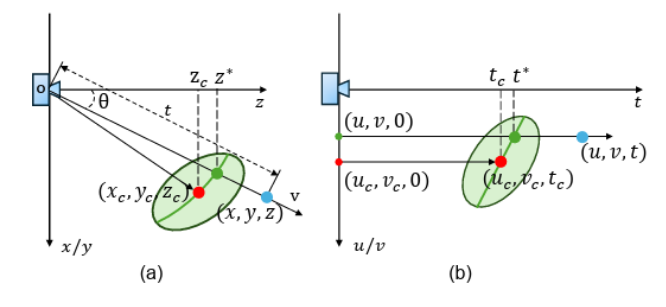
\includegraphics[width=1\linewidth]{../imagenes_marco_teorico/orden_profundidad_espacios.png}
    \caption{En (a), tenemos el espacio de la cámara. En (b), el espacio de rayos. La curva verde representa el conjunto de intersecciones con diferentes rayos de luz.}
    \label{espacio_rayos_camara}
\end{figure}

Notemos que los rayos de luz tienen vector director $(0,0,1)^T$ en el espacio de rayos.

Al transformar las gaussianas, tenemos funciones del tipo

\begin{equation}
G'(u) = e^{-(u-u_c)^T   \Sigma'^{-1}   (u-u_c)}
\end{equation}
con $u$ un punto en el espacio de rayos, $u_c$ y $\Sigma'$ la media y matriz de covarianzas transformadas, respectivamente. Notamos $u_c = (u_c, v_c, t_c)^T$. La matriz de covarianzas es la misma que calculamos anteriormente.

De forma análoga, el máximo se encuentra en

\begin{equation}
t^* = \frac{v'^T \Sigma'^{-1} (u_c - u_o)}{v'^T \Sigma'^{-1} v'}
\end{equation}

Pero, en este caso, la dirección $v'$ es el vector $(0,0,1)^T$, por lo que podemos precomputar $v'^T \Sigma'^{-1} v'$ y $v'^T \Sigma'^{-1}$ para cada gaussiana. Así, el punto de intersección lo podemos reescribir como

\begin{equation}
t^* = \hat{q}(u_c-u_o)
\end{equation}

Como podemos ver a partir de la figura \ref{espacio_rayos_camara}, $t$ es la distancia entre el punto tridimensional $x$ y el centro de la cámara $o$. Así que la profundidad de $x$ es
\begin{equation}
d = cos\theta \cdot t^*
\end{equation}

con $\theta$ el ángulo entre el rayo de luz y el eje principal de la cámara. Para simplificarlo, \cite{zhang2024radegs} aproxima por $\theta_c$, el ángulo definido por la media $x_c$ de la gaussiana. Así, la profundidad $x$ es
\begin{equation}
d = cos\theta_c \cdot t^* = \frac{z_c}{t_c} t^* = \frac{z_c}{t_c} \hat{q} (u_c - u_o)
= \hat{p}(u_c - u_o)
\end{equation}
tomando $\hat{p} = \frac{z_c}{t_c} \hat{q}$ constante para cada gaussiana.

Luego, podemos reformular la ecuación una vez más como
\begin{equation}
d = \hat{p}(u_c - u_o) = \hat{p}(u_c-u,v_c-v,t_c) = \hat{p}(0,0,t_c) + \hat{p}(u_c-u, v_c-v,0)
\end{equation}

El primer sumando, podemos simplificar:

\begin{equation}
\hat{p}(0,0,t_c) = \frac{z_c}{t_c}\hat{p}(0,0,t_c) = \frac{z_c}{t_c} \frac{v'^T \Sigma'^{-1}}{v'^T \Sigma'^{-1}v'} (0,0,t_c) = \frac{z_c}{t_c} \frac{v'^T \Sigma'^{-1}}{v'^T \Sigma'^{-1}v'} (t_c v')
= \frac{z_c}{t_c} \frac{v'^T \Sigma'^{-1} v'}{v'^T \Sigma'^{-1}v'} t_c = z_c
\end{equation}

En el segundo sumado, como el tercer elemento del vector derecho es 0, podemos saltear el tercer elemento de $\hat{p}$, obteniendo el $p$ que buscábamos.

Notemos que, en esta deducción, se introdujo un error al aproximar $\theta$ por $\theta_c$, pero este es despreciable debido a que la proyección local de una gaussiana es pequeña en una imagen dada. Así, los rayos tienen ángulos muy similares, por lo que no es necesario ajustar cuentas posteriores para tener en cuenta este error.

\subsection{Función de costo y gradientes}

Al tratarse de un problema de optimización, es necesario definir una función de costo que permita mejorar la calidad de la reconstrucción iterativamente. Esta función de costo varía en la literatura, pero comúnmente se compone del error fotométrico entre la imagen renderizada y la imagen observada, junto con términos de regularización que imponen restricciones sobre lo parámetros para controlar la estructura de la escena reconstruida.

Sea $\mathcal{L}$ la función de costo a minimizar, se calculan analíticamente los siguientes gradientes de $\mathcal{L}$ respecto de los parámetros de cada gaussiana:

\begin{itemize}
    \item \textbf{Gradiente de color:} Mide cómo ajustar el color de cada gaussiana para reducir la discrepancia entre la imagen renderizada y la observada.
    
    \item \textbf{Gradiente de opacidad:} Indica cómo modificar la transparencia de cada gaussiana para mejorar la correspondencia fotométrica.
    
    \item \textbf{Gradiente de media:} Permite ajustar la posición de cada gaussiana en el espacio tridimensional para mejorar la reconstrucción geométrica.
    
    \item \textbf{Gradiente de covarianza:} Informa sobre cómo modificar la forma y orientación de cada gaussiana para capturar mejor los detalles de la escena. Este se puede descomponer en gradientes de rotación y escala debido a la parametrización de la covarianza, permitiendo mantener la propiedad de semidefinida positiva durante la optimización y manteniendo su interpretación geométrica.


\end{itemize}

\subsection{Gestión de mapa}

Al renderizar imágenes a partir de los splats, existen zonas que podrían quedar subrepresentadas o sobrerepresentadas. Este problema está relacionado tanto con la posición como con la cantidad de gaussianas involucradas. Estas zonas tienen gradientes de posición elevados, lo cual se podría explicar con que la optimización trata de mover las gaussianas para corregir la reconstrucción local. Se identifican estos casos cuando el gradiente de posición supera un umbral, experimentalmente 0.0002.

Es posible mantener constantes las gaussianas y permitir que el algoritmo itere cuanto sea necesario, sin embargo, se obtienen mejores resultados empleando lo que se llama un control adaptativo:

\begin{itemize}
    \item Para las zonas subrepresentadas, tenemos gaussianas pequeñas que no logran representar la geometría local. La densificación, proceso por el cual se agregan gaussianas nuevas, se realiza clonando las gaussianas tales y moviendo la copia en el sentido del gradiente de posición. Al hacer esto, aumenta el volumen cubierto por las gaussianas, y la cantidad de las mismas.

    \item Para las zonas sobrerepresentadas, tenemos gaussianas con gran varianza, cubriendo áreas de elevado tamaño. En este caso, la densificación es a partir de la partición en dos gaussianas, dividiendo la escala por un factor $\phi = 1.6$ determinado experimentalmente. La posición de las dos resultantes se obtiene muestreando sobre la función de probabilidad de la gaussiana original. En este caso, el volumen cubierto por las gaussianas es el mismo, pero aumenta la cantidad.
\end{itemize}

\begin{figure}[H]
    \centering
    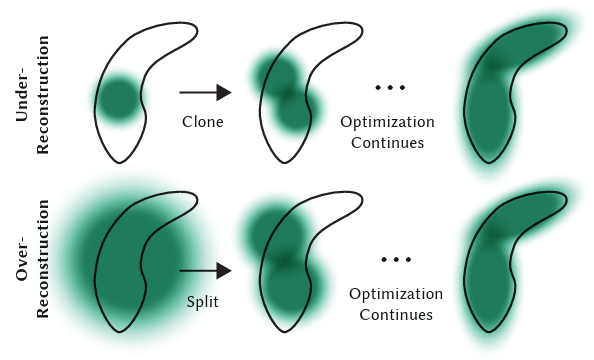
\includegraphics[width=0.75\linewidth]{../imagenes_marco_teorico/densificacion_gaussianas.png}
    \caption{Arriba, se observa la densificación en zonas subrepresentadas clonando la original. Abajo, tenemos la densificación en zonas sobrerepresentadas mediante la partición de la original. Imagen extraída de \cite{zhang2024radegs}}
\end{figure}

Por otro lado, la optimización de los parámetros podría dar lugar a gaussianas con $\alpha$ tan pequeño que su aporte en la representación sea fundamentalmente nulo. Debido a esto, otro paso para el control de gaussianas es la poda, eliminando aquellas con un $\alpha < \epsilon_\alpha$, siendo $\epsilon_\alpha$ un umbral.

Finalmente, el último criterio que se emplea para eliminar gaussianas es calcular la probabilidad de que se considere un \textit{outlier}, i.e., para cada píxel en el que participa durante la rasterización, si la gaussiana modela que el punto se encuentra arbitrariamente más cerca de lo medido, aumenta la probabilidad de ser \textit{outlier}. Experimentalmente, el criterio usa $<0.8d$ con $d$ la distancia medida. Luego, se obtiene la proporción de veces que fue \textit{outlier} para comparar con un umbral inferior, tal que si lo supera es removida.

En este trabajo se exploran distintas heurísticas para la gestión de mapa, las cuales afectarán la densificación de zonas subrepresentadas.




